\documentclass[../../full]{subfiles}


\begin{document}
    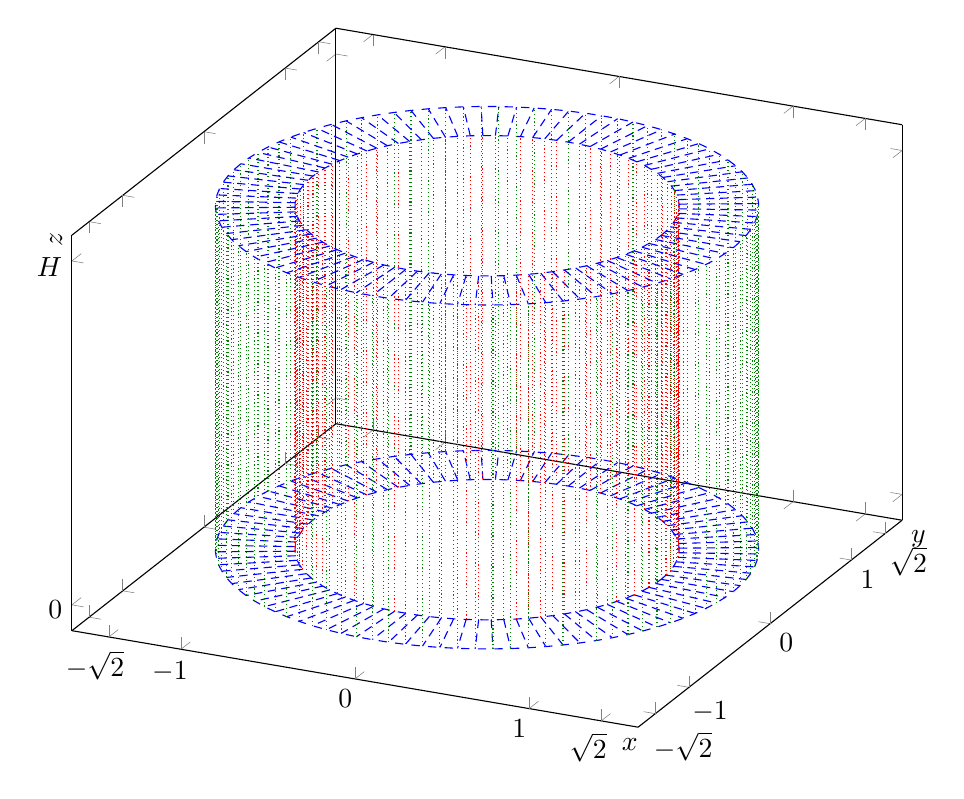
\begin{tikzpicture}
        % colors
        \def\ColorInner{Red}
        \def\ColorOuter{Green}
        \def\ColorFrame{Blue}
        % graphing
        \def\AngleParts{96}
        \def\zHeight{3}
        %
        \begin{axis}[
            width=\textwidth,
            view={25}{30},
            xlabel={\( x \)},
            ylabel={\( y \)},
            zlabel={\( z \)},
            xmin=-sqrt(2), xmax=sqrt(2),
            xtick={-sqrt(2), -1, 0, 1, sqrt(2)},
            xticklabels={\( -\sqrt{2} \), \( -1 \), \( 0 \), \( 1 \), \( \sqrt{2} \)},
            ymin=-sqrt(2), ymax=sqrt(2),
            ytick={-sqrt(2), -1, 0, 1, sqrt(2)},
            yticklabels={\( -\sqrt{2} \), \( -1 \), \( 0 \), \( 1 \), \( \sqrt{2} \)},
            zmin=0, zmax=\zHeight,
            ztick={0, \zHeight},
            zticklabels={\( 0 \), \( H \)},
            enlargelimits=0.075,
            every axis x label/.append style={at=(ticklabel* cs:1)},
            every axis y label/.append style={at=(ticklabel* cs:1)},
            every axis z label/.append style={at=(ticklabel* cs:1)},
        ]
            % circular paths
            \def\LowerInner{}
            \def\LowerOuter{}
            \def\UpperInner{}
            \def\UpperOuter{}
            \foreach \i [
                    evaluate=\i as \Angle using (360/\AngleParts*\i),
                    evaluate=\Angle as \InnerX using cos(\Angle),
                    evaluate=\Angle as \OuterX using (sqrt(2)*cos(\Angle)),
                    evaluate=\Angle as \InnerY using sin(\Angle),
                    evaluate=\Angle as \OuterY using (sqrt(2)*sin(\Angle)),
            ] in {0, ..., \AngleParts} {
                \global\edef\LowerInner{\LowerInner (\InnerX, \InnerY, 0)}
                \global\edef\UpperInner{\UpperInner (\InnerX, \InnerY, \zHeight)}
                \global\edef\LowerOuter{\LowerOuter (\OuterX, \OuterY, 0)}
                \global\edef\UpperOuter{\UpperOuter (\OuterX, \OuterY, \zHeight)}
            }
            \addplot3 [\ColorFrame, no marks, dashed]
                coordinates {\LowerInner};
            \addplot3 [\ColorFrame, no marks, dashed]
                coordinates {\UpperInner};
            \addplot3 [\ColorFrame, no marks, dashed]
                coordinates {\LowerOuter};
            \addplot3 [\ColorFrame, no marks, dashed]
                coordinates {\UpperOuter};
            % straight line paths
            \foreach \i [
                    evaluate=\i as \Angle using (360/\AngleParts*\i),
                    evaluate=\Angle as \InnerX using cos(\Angle),
                    evaluate=\Angle as \OuterX using (sqrt(2)*cos(\Angle)),
                    evaluate=\Angle as \InnerY using sin(\Angle),
                    evaluate=\Angle as \OuterY using (sqrt(2)*sin(\Angle)),
            ] in {1, ..., \AngleParts} {
                \edef\temp{
                    \noexpand \addplot3
                        [\ColorFrame, no marks, densely dashed]
                        coordinates {
                            (\InnerX, \InnerY, 0)
                            (\OuterX, \OuterY, 0)
                        };
                    \noexpand \addplot3
                        [\ColorInner, no marks, densely dotted]
                        coordinates {
                            (\InnerX, \InnerY, 0)
                            (\InnerX, \InnerY, \zHeight)
                        };
                    \noexpand \addplot3
                        [\ColorOuter, no marks, densely dotted]
                        coordinates {
                            (\OuterX, \OuterY, 0)
                            (\OuterX, \OuterY, \zHeight)
                        };
                    \noexpand \addplot3
                        [\ColorFrame, no marks, densely dashed]
                        coordinates {
                            (\InnerX, \InnerY, \zHeight)
                            (\OuterX, \OuterY, \zHeight)
                        };
                }
                \temp
            }
        \end{axis}
    \end{tikzpicture}
\end{document}
